\begin{figure}[htbp]
	\centering
	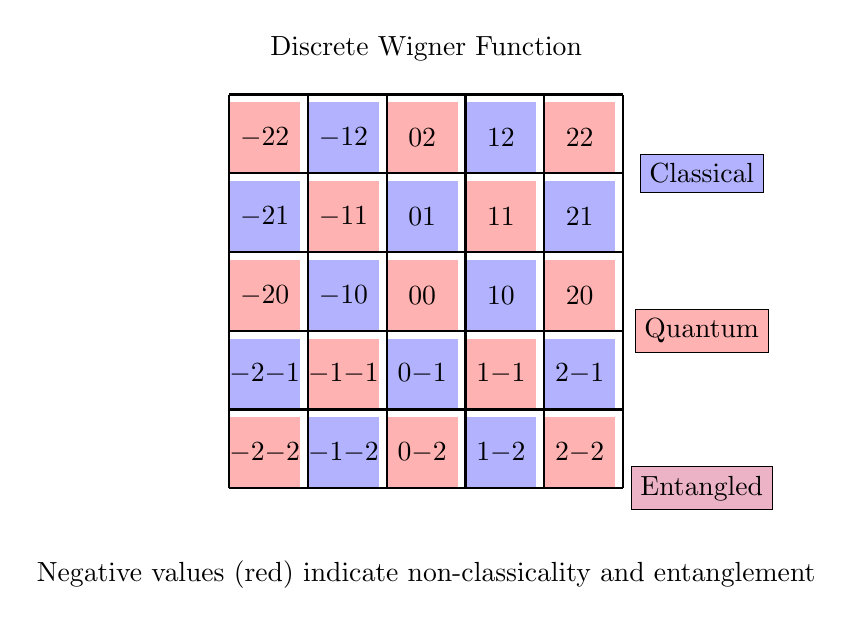
\begin{tikzpicture}
		\foreach \x in {-2,-1,0,1,2} {
				\foreach \y in {-2,-1,0,1,2} {
						\pgfmathparse{\x+\y}
						\ifodd \pgfmathresult
							\fill[blue!30] (\x*1cm,\y*1cm) rectangle ++(0.9cm,0.9cm);
						\else
							\fill[red!30] (\x*1cm,\y*1cm) rectangle ++(0.9cm,0.9cm);
						\fi
						\node at (\x*1cm+0.45cm,\y*1cm+0.45cm) {\pgfmathprintnumber{\x}\pgfmathprintnumber{\y}};
					}
			}
		\draw[thick] (-2cm,-2cm) grid (3cm,3cm);

		\node[draw, fill=blue!30, minimum width=1.5cm] at (4,2) {Classical};
		\node[draw, fill=red!30, minimum width=1.5cm] at (4,0) {Quantum};
		\node[draw, fill=purple!30, minimum width=1.5cm] at (4,-2) {Entangled};

		\node[above] at (0.5,3.3) {Discrete Wigner Function};
		\node[below] at (0.5,-2.8) {Negative values (red) indicate non-classicality and entanglement};
	\end{tikzpicture}
	\caption{Discrete Wigner function for a qubit system. Each cell represents a phase space cell, with colors indicating quasi-probability values. Negative values (red) signal non-classicality.}
	\label{fig:wigner-function}
\end{figure}
